\section{Discussion and Outlook}\label{sec:disc}

In this tutorial, we have presented a brief overview of the current techniques for rule induction from knowledge graphs and have demonstrated how reasoning over KGs using the learned rules  can be exploited for KG completion. % discussed the different approaches for rule induction and reasoning over real-life KGs. We briefly illustrated the common method for KG construction and the incompleteness and inaccuracy challenges they face. We also illustrated the difference between \textit{Horn} and  \textit{nonmonotonic} logic program and their connection to association rules. Later, we reviewed some of the existing systems for constructing Horn rules from KGs and the proposed rule evaluation measurements under OWA. Furthermore, we discussed the exiting inductive and abductive methods for learning nonmonotonic rules and their applicability over real-life KGs. Finally, we discussed rule revision approach RUMIS, which tries to capture exceptional cases to achieve accurate and consistent predictions. 

While the problem of rule-based KG completion has recently gained a lot of attention, several promising research directions are still left unexplored. % Despite the advances in rule learning, the existing methods still learn limited formats for rules, \eg closed rules, with even restrictive language bias.
% Additionally, they are still prone to KG incompleteness and not being able to determine the possible gaps in the data under OWA. These challenges lead to the generation of uninteresting and noisy rules. Follows some possible directions to overcome such challenges. 

\leanparagraph{Learning Other Rule Forms}
%Prominent rule learning approaches only extract normal $closed$ logical rules, which may not capture all interesting patterns. However, 
While the majority of available methods focus on extracting Horn or nonmonotonic rules, inducing rules of other forms may be beneficial. These include %other rule forms such as 
disjunctive rules
%(\eg $hasBrother(X,Y) \vee hasSister(X,Y) \leftarrow hasSibling(X,Y)$, or $livesIn(X, north\_korean) \vee livesIn(south\_korean) \leftarrow speaks(X, korean) $),
(e.g., \emph{``Having a sibling implies having a sister or a brother'', ``Korean speakers are normally either from South or North Korea''})
 or rules with existential quantifiers in the head (e.g., \emph{``Being a musicians in a band, implies  playing some musical instrument''}).
%(\eg $\exists Y: playsInstrument(X, Y) \leftarrow$ $musician(X),bandMember(X,Z)$) is an interesting topic to study. 
Several recent works on mining keys in KGs \cite{vickey,DBLP:conf/www/LajusS18}, detecting mandatory relations \cite{DBLP:conf/www/LajusS18} and learning SHACL constraints \cite{shacl} are relevant, but they do not directly address the mentioned rule forms. A combination of techniques from relational rule learning \cite{DBLP:books/daglib/0021868} and propositionalization approaches \cite{propos} can be utilized for learning rules with existentials, yet it is unclear how to detect KG parts that are worth propositionalizing and combine the outputs of both methods.  % can encode more interesting patterns
% Even though these
% While rules with existential variables in the head may not directly infer new facts, they may reflect interesting patterns in the data and, moreover, can be used as a guidance for the information retrieval approaches and crowd-sourcing.

Rules that reflect correlations between edge counts in KGs such as \emph{``If a person has two siblings then his/her parents are likely to have 3 children''} have been studied in \cite{carl}. Inducing more general rules, encoding mathematical functions on edge counts (e.g.,  \emph{``If a person has k siblings then his/her parents are likely to have k+1 children''}) and other numerical rules is still an open problem, which is particularly challenging due to large search space of possible hypothesis.

% \leanparagraph{Learning temporal rules} 
% Current approaches extract the rules from the directly stated entities and relations. More promising direction would be to learn patterns over more unstated relations such as temporal rules. For examples, KGs usually contain the dates of the events, \eg $\mi{dateOfbirth}$ or $happenedOn$ which is sparse data and requires arithmetic operator to make use of them, \eg $before(X,Y)$, $after(X,Y)$. Learning interesting rules over this data is still not well studied.
Learning temporal rules or constraints such as \emph{``A person cannot graduate from a university before being born''} is another promising future work direction. Deductive reasoning over temporal KGs has been recently considered in \cite{DBLP:conf/aaai/ChekolPSS17}; however, the inductive setting has not yet been studied in full details to the best of our knowledge. A framework for learning hard boolean constraints has been described in \cite{DBLP:conf/aaai/RaedtPT18}, but its extension to KGs and soft constraints is still missing. 

\leanparagraph{Learning Rules from Probabilistic Data}  %Nevertheless, e
The majority of existing rule learning approaches over knowledge graphs model KGs as sets of true triples thus totally ignoring possible inaccuracy of some of the facts that they encode. Since KGs are normally automatically constructed from noisy textual resources, obviously not all of the extracted facts should have the same weight. Learning rules from such noisy KGs by treating all facts equally might naturally lead to problematic rules, which when applied could propagate faulty facts. 

A recent ILP approach that accounts for noise has been proposed in \cite{sigmailp}; but it relies on CWA and neglects weights on the facts.
Learning rules from KGs treated as uncertain data sources has  been considered in \cite{probfoil,DBLP:conf/ijcai/RaedtDTBV15,DBLP:conf/clima/CorapiSIR11}; however, these works neglect negation, disjunction or existential variables in the head. %  reduce the effect of inaccurate facts in the KG 
Extending the techniques to more advanced rule forms is desired.

 %Addressing the rule learning over weighted data has been studied under probabilistic ILP%, where given a set of probabilistic examples for grounded atoms and a target predicate $H$, the task is to learn rules for predicting probabilities of atoms for $H$
% However, exploiting these techniques in our setting requires a full materialization of the probability function,
% which quickly grows to sizes that ILP methods cannot handle. Adapting probabilistic rule learning approaches for real-life KGs has only been studied in~\cite{DeRaedt:2015}, leaving a wide room for improvements.

\begin{figure}[t]
\centering
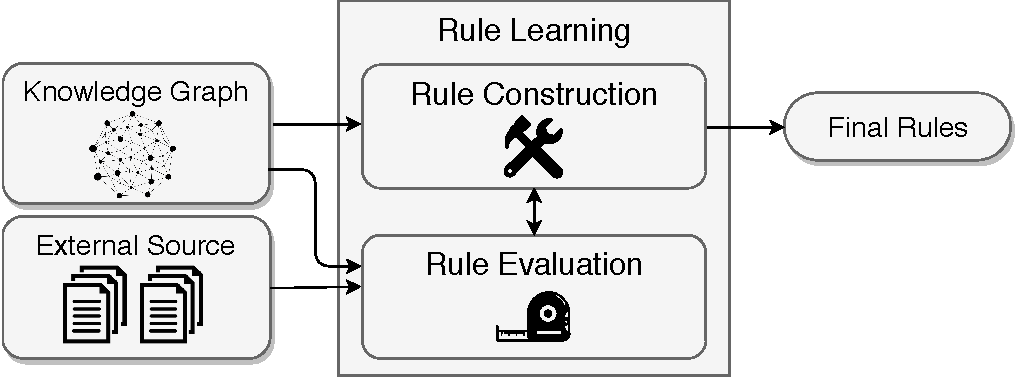
\includegraphics[width=8cm]{figures/discussion_overview}
\caption{Rule learning with external sources.}
\label{fig:discussion_overview}
\end{figure}


\leanparagraph{Rule Learning with External Sources} 
Another interesting research stream is to consider pieces of evidence from hybrid external sources while inducing rules from KGs
(see Figure~\ref{fig:discussion_overview}). Similar to \cite{DBLP:conf/rweb/EiterKRSW17}, where external functions are utilized during deductive reasoning, various heterogeneous information sources can be used to guide rule induction. These range from a human expert giving feedback about the correctness of a given rule (similar as done in \cite{Dzyuba2017} for pattern mining), to dedicated fact-checking engines (e.g., Defacto~\cite{defacto}, FactChecker~\cite{factchecker}) that given a fact such as $\mi{bornIn(einstein,ulm)}$ rely on Web documents to estimate its truthfulness. 
%This amounts to utilizing such automated fact-checking systems as  in the rule induction process. 

%An alternative relational learning method for KG completion is to learn representations (i.e. embeddings) of entities and relations from a given KG possibly enriched with additional information sources (e.g., text) with the % propose
%purpose of estimating the likelihood of unseen facts (see \cite{Wang2017} for overview). However, the
%predictions produced by such approaches are not interpretable~\cite{Shakerin2018}. Interlinking these statistical methods with inductive rule learning is a promising further direction.

\leanparagraph{Neural-based Rule Learning} Utilizing embedding models for rule learning is a new research direction that has recently gained attention \cite{DBLP:conf/nips/YangYC17,DBLP:journals/corr/YangYHGD14a}. Existing methods are purely statistics-based, i.e., they reduce the rule learning problem to algebraic operations on neural-embedding-based representations of a given KG. The approach \cite{DBLP:journals/corr/YangYHGD14a} constructs rules by modeling relation composition as multiplication or addition of two relation embeddings. The authors of \cite{DBLP:conf/nips/YangYC17} propose a differentiable system for learning models defined by sets of first-order rules that exploits a connection between inference and sparse matrix multiplication \cite{DBLP:journals/corr/Cohen16b}. However, existing approaches pose strong restrictions on target rule patterns, which often prohibit learning interesting rules, e.g. non-chain-like or exception-aware ones. Combining neural methods with symbolic ones and accounting for rich background knowledge in the form of logical theories is expected to be advantageous for obtaining surprising insights from the data.


%\leanparagraph{Hybrid rule learning techniques}
 \leanparagraph{Extracting Rules Jointly from KGs and Text} While modern KGs are rich in facts and typically rather clean, they contain a limited set of encyclopedic relations (e.g., $\mi{bornIn}$, $\mi{marriedTo}$). On the other hand, textual resources certainly cover a richer set of predicates (e.g., $\mi{gotAquintedWith}$, $\mi{celebratedWedding}$), but suffer from  noise. % Extracting logic rules from text using natural language processing (NLP) techniques and textual entailment has been studied in several works~\cite{Schoenmackers:2010,Gordon:2011,dragoni2016}.  
%these methods only depend on the noisy information that exists in the text. 
A natural way to address the %One way to address this, is by  %overcome the noise while extracting rules is to utilize 
above issues is to combine 
%utilizing KG facts %while processing the text 
%jointly with textual sources (\ie in the form of a semantic mark-up) % as proposed in
%. Development of methods that combine 
 %Combining these %linguistics-based 
text-based rule extraction relying on natural language processing (NLP) and textual entailment techniques~\cite{Schoenmackers:2010,Gordon:2011,dragoni2016} with inductive rule learning from KGs. This interesting research direction comes with many challenging due to the heterogeneity of the input sources.
  %has a great potential % Indeed,
%has a great potential. %for overcoming the limited KG scope.
%the restrictions imposed due to the limited number of predicates in most encyclopedic KGs. Hence, obtaining more interesting and accurate rules. 
% For example, rules learned from a KG only about the marriage relationship between two persons usually rely on the existence of $hasChild$ or $livesIn$ relation, to a common child or place respectively, in the KG.

%  \[ \mi{isMarriedTo(X,Y)} \leftarrow \mi{hasChild(X,Z),hasChild(X,Z)}\]
%  \[\mi{isMarriedTo(X,Y)} \leftarrow \mi{livesIn(X,Z),livesIn(X,Z)}\]
% while these rules are statistically correct, they are not always accurate when used to predict new facts. Observing more information in text such as ``they celebrated their wedding in ...'' can increase the precision of the predictions. This textual evidence can be %induced in 
% injected into the rules using higher-arity predicates such as  
% \begin{align*}
%  \mi{isMarriedTo(X,Y)} \leftarrow &\mi{hasChild(X,Z),hasChild(X,Z)},\\ &\mi{textEvidence(isMarriedTo,X,Y)}
% \end{align*}
% The textual evidences can be of various forms including %be either 
% ``a bag of words'' or a context correlated with the target predicates.
% Such 
%The discussed research direction is promising %has a good potential 
%for enhancing the predictive  quality of learned rules. 
%for predicting new facts.
 %\gad{I am thinking of some example} 

 % is rather limited, since they are primarily extracted from Wikipedia; this prohibits the extraction of many interesting rule patterns such as ``\ds{TODO: insert. The previous rule about injured people has a negative flavor for being in the end of the article and it needs more motivation}''. %, like % where such non-standard facts as ``Einstein worked with Feynmen'' are rarely added. The number of predicates is limited in most of the KGs. Therefore, sometimes it is hard to learn interesting patterns from the KG only. In contrast, textual resources are rich with verbal phrases that indicate events or relations. However, learning the simplest rules from unstructured resources is challenging. Therefore, it worth investigating constructing hybrid rules that combine both resources.  For example, to learn a rule such as

% \begin{align*}
% \mi{participatedIn(X,Y)} \leftarrow & \mi{playsFor(X,Z)}, \mi{competes(Z,Y)},\\ & \naf injuredDuring(X,Y)
% \end{align*}
% \ds{would suggest to add a different rule here, this }
% The rule encodes that a player participates in a championship if he plays for a competing team unless he was injured during the championship. Learning the positive part of the rule can be easily done over the KG, yet the last one is more common to find in the text. 




%\section{Discussion and Outlook}
%\label{sec:discussion_outlook}
%Toward the rule-based KG completion problem, a number of future directions could be put into consideration.
%\subsubsection{Rule Learning with External Source.}

%In most of rule learning systems have been proposed \cite{amie,op,rdf2rules}, while their rule construction methods may vary, the core of them is at the proposed rule evaluation metric. Various rule measures have been introduced, from the simplest to the most sophisticated one. Nevertheless, most of them are computed based on only the given graph, and cover only a small subset of local patterns in the KG, thus might wrongly estimate the quality of extracted rules since real-world KGs are usually highly incomplete.
%
%One promising possibility to tackle this problem is to incorporate external related data from outside of the KG. The overview of such rule learning system could be described in Figure \ref{fig:discussion_overview}. The KG related external data can be extracted from many sources (e.g. crowd-sourcing, Web-extraction), and is obviously useful not only for rule evaluation, but also for rule construction over the KG. For instance, external data can give some feedback about the quality of predicted facts in several forms such as binary decision (\ie true or false) or a likelihood score. This feedback could be then taken into account for rule quality evaluation or exception capturing. In addition, external KG meta-data could gives some information about the existence of certain types of facts within the KG (as exploited in CARL~\cite{carl}). Moreover, we can also somehow learn rules directly from the text and then apply them back to the KG.
%
%An alternative relational learning method for KG completion is to learn representations (i.e. embeddings) of entities and relations for predicting likelihood of unseen facts. While these methods capture global patterns in the data, the predictions that they produce are not interpretable~\cite{Shakerin2018}. Many such models are been proposed \cite{Wang2017}, in which some of them could even be extended with additional unstructured knowledge (e.g., text corpus). Hence, integrating these embedding models into the rule learning approach might be a potential solution for the problem of rule-based KG completion.
%\subsubsection{Learning Various Rule Forms}
%In the KG completion problem, as mentioned, most of the rule mining approaches only mine $closed$ rules. Nevertheless, other form of rules might be also interesting. For example, rules with disjunction (e.g. $isMale(X) \vee isFemale(X) \leftarrow isPerson(X)$), rules with quantifier (e.g. $(\exists Y: playsInstrument(X, Y)) \leftarrow isMusician(X))$). Even though these kinds of rule do not directly make predictions on the knowledge graph since we do not know exactly which facts of the head are true, they might give us some useful constraints about the knowledge graph.
